\section[I modelli]{I modelli}
\label{sec:models}
\sectionframe{images/covers/cover_architecture.jpeg}{I modelli}	


\subsection[I componenti essenziali]{I componenti essenziali}
\begin{frame}
	\frametitle{I componenti essenziali}
	
	\begin{block}{I componenti essenziali}
		Adesso che abbiamo chiarito quali siano i principali componenti elettronici che formano un computer, definiamo quali sono i componenti essenziali di un computer:
		\begin{itemize}
			\item il processore
			\item la memoria
			\item l'input/output (I/O)
		\end{itemize}
		
	\end{block}
	
\end{frame}



%\begin{frame}
%	\frametitle{L'architettura di un computer}
%	
%	\begin{block}{L'architettura di un computer}
%		In generale, l'architettura di un computer può essere divisa in tre parti principali:
%		\begin{itemize}
%			\item il processore
%			\item la memoria
%			\item l'input/output (I/O)
%		\end{itemize}
%	\end{block}
%	
%%	\begin{figure}[!htbp]
%%		\centering 
%%		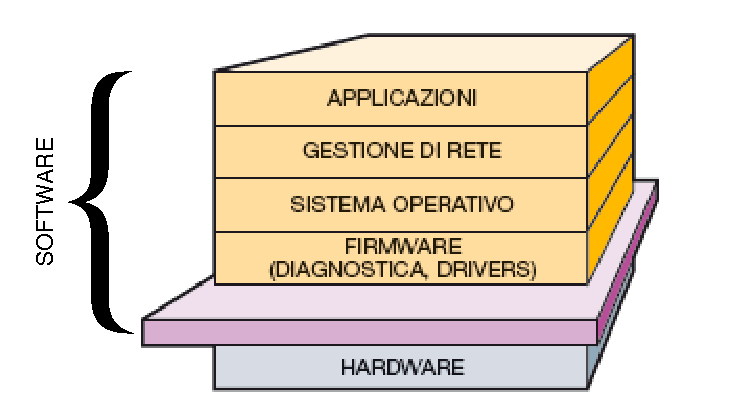
\includegraphics[width=0.6\linewidth]{images/3_modelli/hd-sw.pdf}
%%%			\caption{}
%%	\end{figure}
%	
%\end{frame}


\subsubsection[Il processore]{Il processore}
\begin{frame}
%	\frametitle{L'architettura di un computer}
	
	\begin{block}{Il processore}
		Il \textbf{processore}, noto anche come "microprocessore", è il "cervello" del computer, ed è responsabile dell'esecuzione delle istruzioni contenute nel software.
	\end{block}

	\begin{columns}			
		\column{0.5\linewidth}
		\begin{figure}[!htbp] 
			\centering
			%\advance\leftskip-0.25cm
			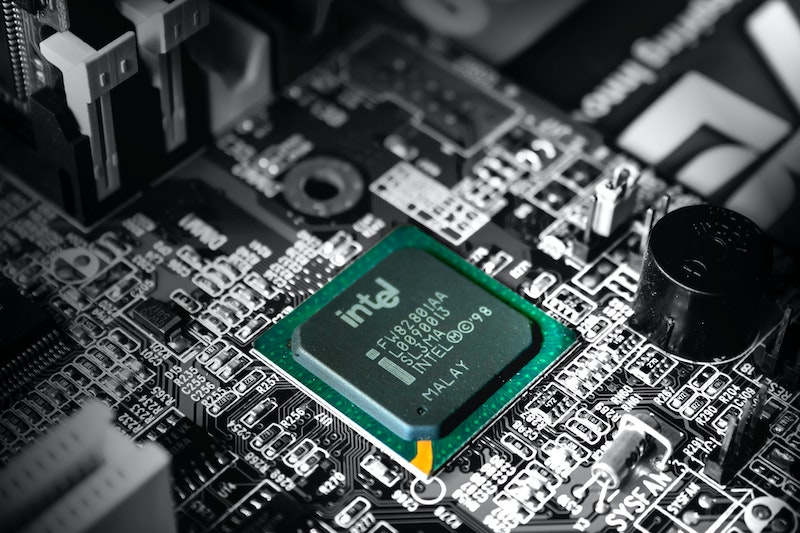
\includegraphics[width=1.0\linewidth]{images/3_modelli/intel.jpg}
			\caption{Processore Intel}
			\label{fig:models_intel}
		\end{figure}
					
		\column{0.5\linewidth}
		\begin{figure}[!htbp] 
			\centering
			%\advance\leftskip-0.25cm
			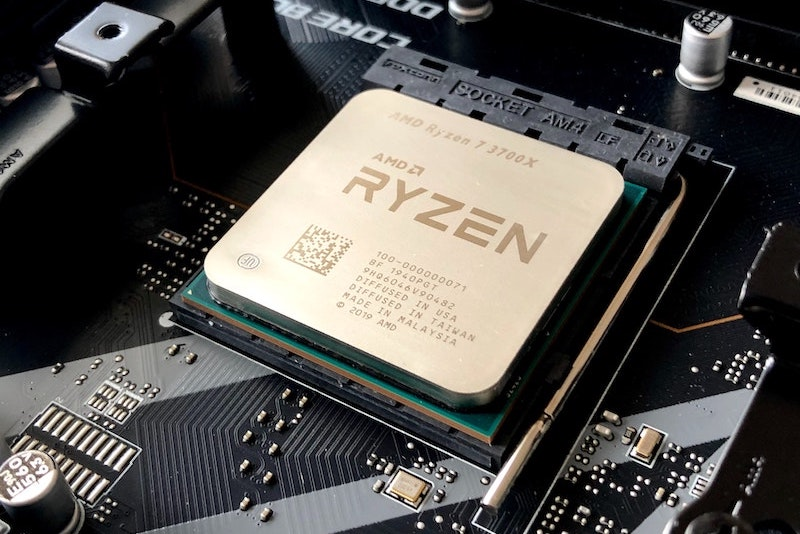
\includegraphics[width=1.0\linewidth]{images/3_modelli/ryzen.jpg}
			\caption{Processore AMD Ryzen}
			\label{fig:models_ryzen}
		\end{figure}
		
	\end{columns}
	
\end{frame}



\subsubsection[La memoria]{La memoria}
\begin{frame}
%	\frametitle{L'architettura di un computer}
	
	\begin{block}{La memoria}
		La \textbf{memoria} è dove vengono temporaneamente archiviati i dati e le istruzioni che vengono utilizzati dal processore. Esistono due tipi principali di memoria: 
		\begin{itemize}
			\item la \textbf{memoria RAM} (Random Access Memory), che viene utilizzata per archiviare i dati che il processore sta attualmente lavorando
			\item la \textbf{memoria di massa}, come il disco rigido o il solid state drive, che viene utilizzata per archiviare i dati a lungo termine.
		\end{itemize}
	\end{block}
	
	\begin{columns}			
		\column{0.5\linewidth}
		\begin{figure}[!htbp]
			\centering
			%\advance\leftskip-0.25cm
			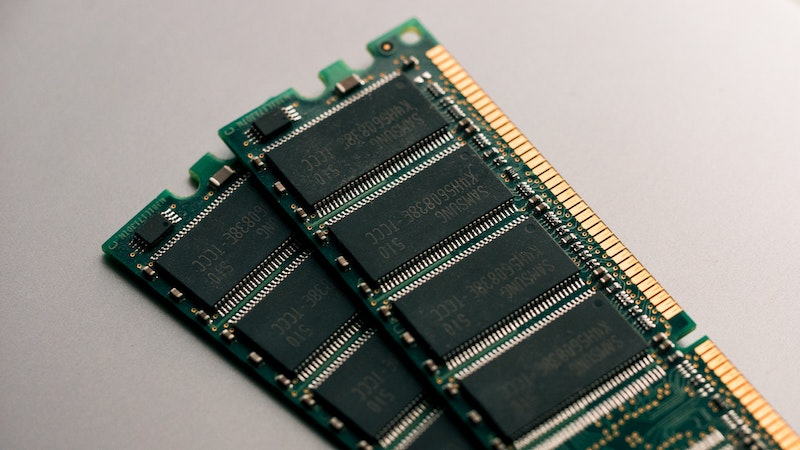
\includegraphics[width=0.82\linewidth]{images/3_modelli/memory_ram.jpg}
			\caption{Due memorie RAM}
			\label{fig:models_memory_ram}
		\end{figure}
					
		\column{0.5\linewidth}
		\begin{figure}[!htbp] 
			\centering
			%\advance\leftskip-0.25cm
			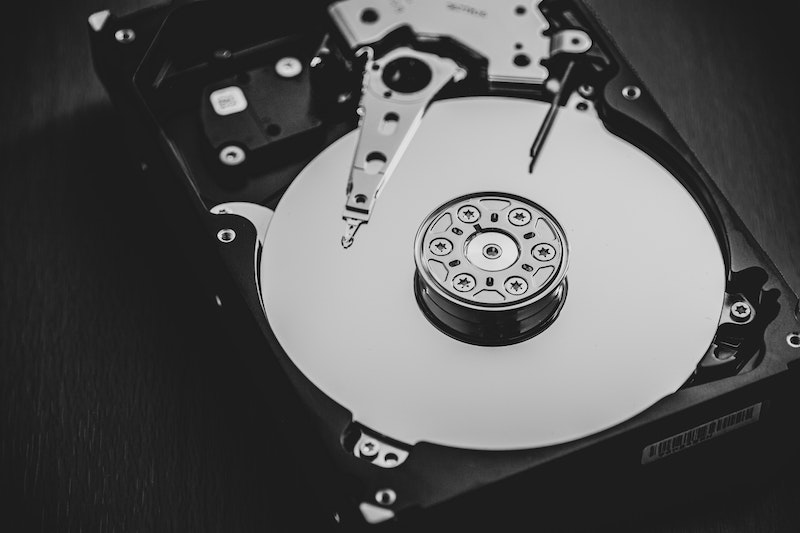
\includegraphics[width=0.7\linewidth]{images/3_modelli/memory_hdd.jpg}
			\caption{L'interno di un Hard Disk}
			\label{fig:models_memory_hdd}
		\end{figure}
		
	\end{columns}
	
\end{frame}


\subsubsection[L'input/output (I/O)]{L'input/output (I/O)}
\begin{frame}
%	\frametitle{L'architettura di un computer}
	
	\begin{block}{L'input/output (I/O)} 
		L'\textbf{input/output} (I/O) gestisce il flusso di dati tra il computer e l'esterno, attraverso dispositivi come il monitor, la tastiera e il mouse.
	\end{block}
	
	\begin{figure}[!htbp] 
		\centering
		%\advance\leftskip-0.25cm
		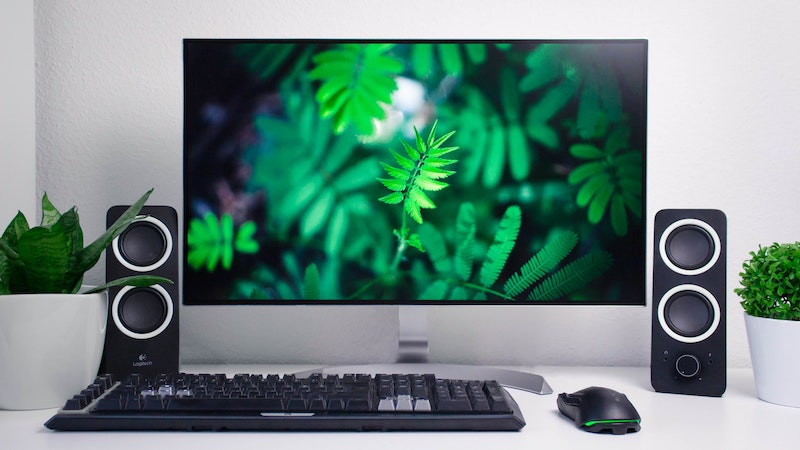
\includegraphics[width=0.8\linewidth]{images/3_modelli/io.jpg}
		\caption{Monitor, tastiera, mouse e casse}
		\label{fig:models_io}
	\end{figure}
	 
\end{frame}


\begin{frame}
%	\frametitle{L'architettura di un computer}
	
	\begin{block}{Altre componenti}
		Altre componenti comuni di un computer possono includere schede di espansione, che forniscono ulteriori funzionalità al computer, come ad esempio la possibilità di collegare dispositivi esterni o di aggiungere ulteriori porte di I/O.
	\end{block}
	
%	\begin{figure}[!htbp]
%		\centering 
%		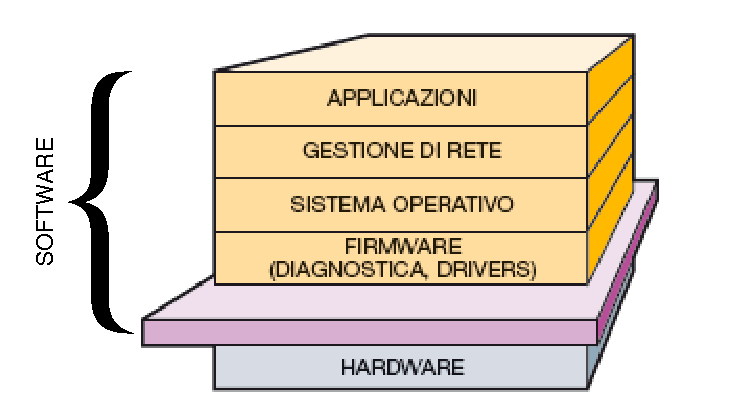
\includegraphics[width=0.6\linewidth]{images/3_modelli/hd-sw.pdf}
%%			\caption{}
%	\end{figure}
	
\end{frame}


\subsection[I modelli]{I modelli}
\begin{frame}
	\frametitle{I modelli}
	
	\begin{block}{I modelli}
		
		I due modelli maggiormente utilizzati per illustrare il funzionamento di massima del sistema-computer sono:
		\begin{itemize}
			\item il \textbf{modello di Von Neumann}
			\item il \textbf{modello di Harvard}
		\end{itemize}
	\end{block}
	
%	\begin{figure}[!htbp]
%		\centering 
%		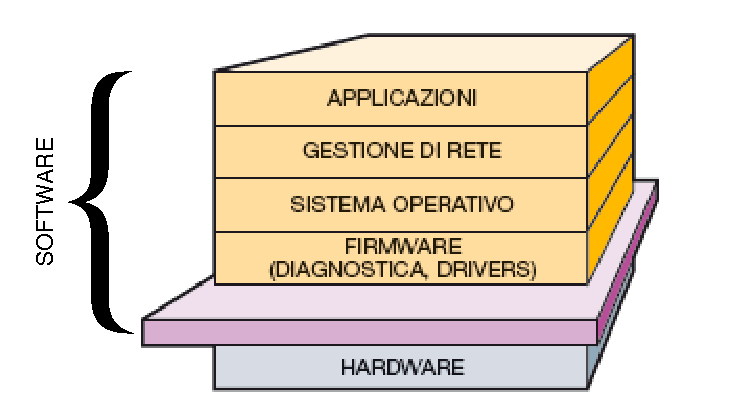
\includegraphics[width=0.6\linewidth]{images/3_modelli/hd-sw.pdf}
%%			\caption{}
%	\end{figure}
	
\end{frame}

\subsubsection[Il modello di Von Neumann]{Il modello di Von Neumann}
\begin{frame}
	\frametitle{Il modello di Von Neumann}
	
	\begin{block}{Il modello di Von Neumann}
	
	\end{block}
	
	
\end{frame}


\subsubsection[Il modello di Harvard]{Il modello di Harvard}

\begin{frame}
	\frametitle{Il modello di Harvard}
	
	\begin{block}{Il modello di Harvard}
	
	\end{block}
	
	
\end{frame}
